% !TeX root = ../main.tex

% Front content of the Dissertation
\title{Secure Smart Lock System}

\author{by\\Zack Pollard\\
\\
{\bf A Final Year Dissertation}\\
\\
Submitted in partial fulfilment of the requirements for the award of\\
BSc Computer Science of Loughborough University\\
\\
\copyright
\hspace{1 dd} Zack Pollard 2018\\
\\
April 2018
}
\date{} % Used to remove date from title so it can be set at any date rather than the current date

%\maketitle

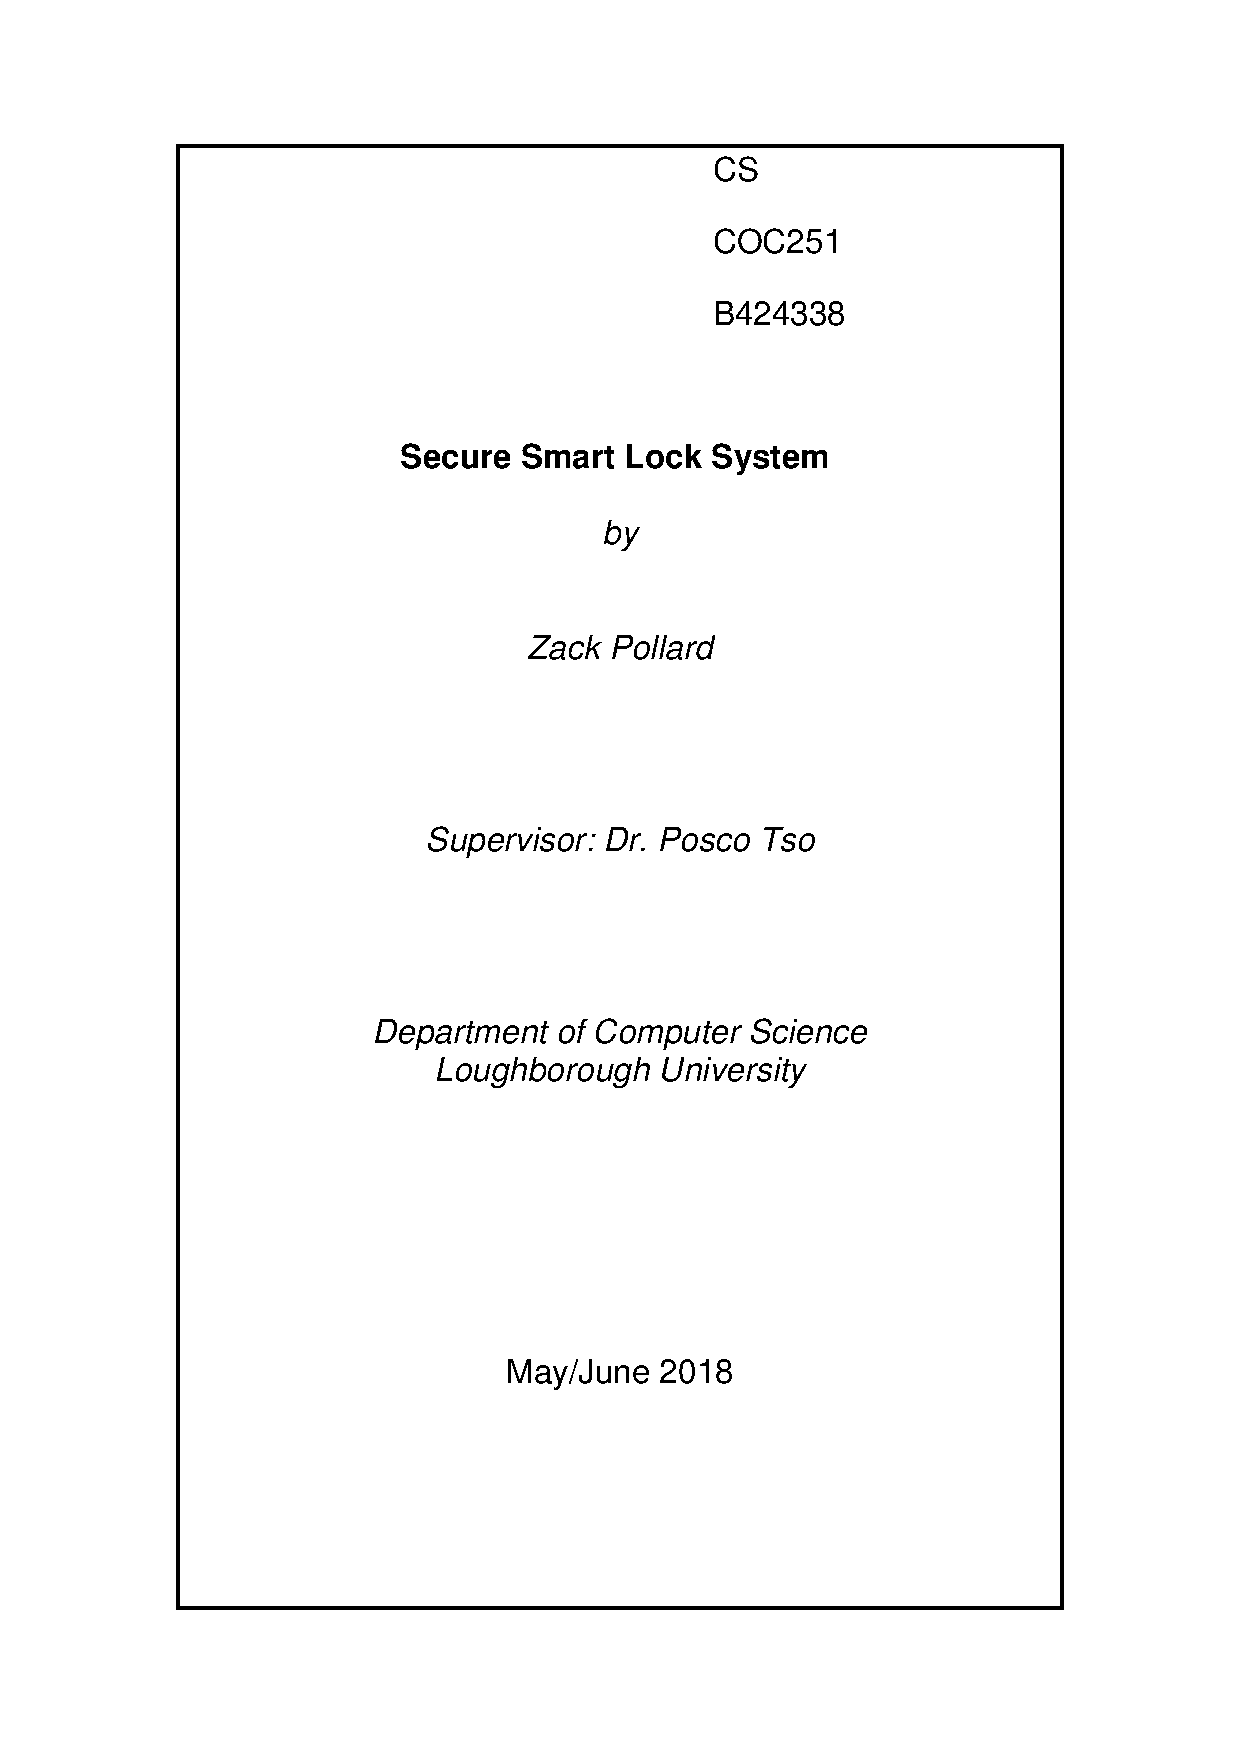
\includepdf{Graphics/frontpage-2018.pdf}

% Set page numbers to roman numerals for front matter
\pagenumbering{roman}

% PDF exports of Word Documents available (Exported August 2012)
% Thesis Access Form
%\includepdf[pages=1, pagecommand=, templatesize={5in}{10in}]{Front/LU/access.pdf}
% Certificate of Originality
%\includepdf[pages=-, pagecommand=, templatesize={5in}{10in}]{Front/LU/origin.pdf}

% Abstract
\chapter*{Abstract}
\addcontentsline{toc}{chapter}{Abstract}
%Include an abstract of your Thesis, should be around 300 words (1 side of A4).
%The abstract immediately follows the title page, and is presented on a page on its own.
%It consists of a brief summary of no more than 300 words which accurately outlines the
%main aims and achievements of your dissertation.

This report covers the creation of a secure smart lock system made up of a central server, a raspberry pi core and an Android application. The idea behind this project is to make a system that is both secure and easy to use, two traits which are generally difficult to combine as generally extra security means extra complexity. The system described within this report demonstrates that it is possible to have security and ease of use side by side using the design that I have laid out.

Initially the report goes over aims and objectives for the user but also for the technical side of the project. This was an important distinction for this project as it has both complex technical and user requirements when put together. Following that a literature review looks at the current smart locks on the market to examine strengths, weaknesses and security exploits in the existing products. Once the research was completed the report moves on to the requirements, design and implementation stages of the report which focus on the product that I have built as well as potential improvements and further possible work that could be done. Finally it goes on to a conclusion covering what I most enjoyed in the project, my strengths and weaknesses throughout and my opinion of the outcome of the project as a whole.


% Acknowledgements
\chapter*{Acknowledgements}
\addcontentsline{toc}{chapter}{Acknowledgements}
%In this section you should acknowledge those who have helped you or offered you advice
%during your project. It is common courtesy to include an acknowledgement to
%your project supervisor. People sometimes also include acknowledgement of family and
%friends who have helped to proof-read the work or provided emotional support. The
%acknowledgement should be brief and succinct.

I want to acknowledge the following people who have provided ongoing support and help throughout the course of this project:
\begin{itemize}
	\item My project tutor, Dr. Posco Tso, for his continued guidance, support and professionalism throughout the project.
	\item My parents for their continued help and support.
	\item My girlfriend, Jessica Benham, for her constant love, encouragement and support throughout.
\end{itemize}

% Set the depth for your table of content
% Currently set at 2 (Chapter, Section, Subsection)
\setcounter{tocdepth}{2}
% Include a table of content
\tableofcontents
%This section should be be entitled “Contents” and should provide a list of chapter,
%section and subsection headings with their appropriate page number. You are strongly
%advised to use the features provided within LATEX or your word-processing software to
%auto-generate this page. This ensures that the details are correct and reduces a lot of
%labour-intensive and painstaking work. An example contents page is provided at the
%start of this document (although you should note that this document is in ‘article’ style
%and therefore not structured with chapters as a dissertation would be).

% Include a list of figures
\listoffigures
\addcontentsline{toc}{chapter}{List of Figures}

\newpage

% Set page numbering to arabic for body of Thesis
\pagenumbering{arabic}